\documentclass[a4paper,twoside,12pt]{report}

\usepackage{fullpage}
\usepackage{float}
\usepackage{url}
\usepackage{charter}
\usepackage{graphicx}
\usepackage{subfigure}
\usepackage{amsmath}
\usepackage{amssymb}
\usepackage{amsthm}
\usepackage{booktabs}
\usepackage{parskip}
\usepackage{algorithm}
\usepackage{algpseudocode}
\usepackage{xcolor}
\usepackage{soul} % provides \hl{...} for highlighting
\usepackage{tikz}
\usepackage{pgfplots}
\usepackage{pgfplotstable}
\pgfplotsset{compat=1.18}
\usetikzlibrary{arrows.meta, positioning, shapes.geometric, fit, backgrounds}
\usepackage[all]{nowidow}
\setnoclub[2]
\setnowidow[2]

% Referencing
\usepackage{varioref}
\usepackage[bookmarks=true,bookmarksopen=true]{hyperref}
\usepackage{cleveref}
\hypersetup{
  colorlinks = true,
  urlcolor   = blue,
  linkcolor  = blue,
  citecolor  = blue
}
\crefname{table}{table}{tables}
\Crefname{table}{Table}{Tables}
\crefname{figure}{figure}{figures}
\Crefname{figure}{Figure}{Figures}
\crefname{equation}{equation}{equations}
\Crefname{equation}{Equation}{Equations}

% Wits Citation Style
\usepackage{natbib} \input{natbib-add}
\bibliographystyle{named-wits}
\bibpunct{[}{]}{;}{a}{}{}
\setlength{\skip\footins}{1.5cm}
\newcommand{\citets}[1]{\citeauthor{#1}'s \citeyearpar{#1}}
\renewcommand\bibname{References}

\pagestyle{plain}
\pagenumbering{roman}

\renewenvironment{abstract}{%
  \ \vfill\begin{center}\textbf{Abstract}\end{center}%
  \addcontentsline{toc}{section}{Abstract}}{\vfill\vfill\newpage}
\newenvironment{declaration}{%
  \ \vfill\begin{center}\textbf{Declaration}\end{center}%
  \addcontentsline{toc}{section}{Declaration}}{\vfill\vfill\newpage}

% Macros
\newcommand{\runsafe}{R_{\text{unsafe}}}
\newcommand{\vmin}{V_{\min}}
\newcommand{\vmax}{V_{\max}}
\newcommand{\rmin}{R_{\min}}
\newcommand{\rmax}{R_{\max}}

% ---- Reusable TikZ styles ---------------------------------------------------
\tikzset{
  block/.style  = {draw, rounded corners, minimum width=2.8cm,
                   minimum height=0.85cm, align=center, font=\small},
  bblue/.style  = {block, fill=blue!10},
  borange/.style= {block, fill=orange!20},
  bred/.style   = {block, fill=red!12},
  bgreen/.style = {block, fill=green!12},
  bgray/.style  = {block, fill=gray!10},
  arr/.style    = {-{Stealth}, thick}
}

% =============================================================================
\begin{document}
\onecolumn
\thispagestyle{empty}
\setcounter{page}{0}
\addcontentsline{toc}{chapter}{Preface}
\ 
\begin{center}
  \vfill
  {\huge\bf\textsc{Safe Reinforcement Learning via Minmax Penalties}\\[20pt]
   \large School of Computer Science \& Applied Mathematics\\
   \large University of the Witwatersrand\\[20pt]
   \normalsize
   Wendy Maboa\\[2pt]
   {2541693}\\[20pt]
   Supervised by Geraud Nangue Tasse\\[10pt]
   \today}
  \vfill\vfill
  
\includegraphics[width=1.5cm]{images/wits}
  \vspace{10pt}\\
  \small{Ethics Clearance Number: XX/XX/XX}\\[10pt]
  \small{A proposal submitted to the Faculty of Science, University of the Witwatersrand,
  Johannesburg, in partial fulfilment of the requirements for the degree of Master of
  Science in Computer Science}\\
\end{center}
\vfill
\newpage

\pagestyle{plain}
\setcounter{page}{1}

% ---- Abstract ---------------------------------------------------------------
\phantomsection
\begin{abstract}
\noindent

Reinforcement Learning (RL) has demonstrated remarkable results, from mastering games
like Atari and Go to shaping the behaviour of Large Language Models (LLMs). Existing
safety alignment frameworks, including KL divergence penalties and learned cost models,
address this challenge but introduce annotation costs, additional hyperparameters, or
resource-intensive components. Moreover, models fine-tuned with these approaches can still
produce harmful content such as hate speech and discriminatory outputs. This research
proposes that a safety signal may already exist within the RL loop itself. Drawing from
the ROSARL algorithm, we adapt its Minmax penalty to the LLM fine-tuning setting,
replacing both the KL divergence penalty and the learned cost model with a
value-function-derived safety signal. This eliminates the need for a separate cost model or
Lagrange multiplier. Proof-of-concept experiments on GPT-2 small and a small Qwen model
(exact size in the 0.5 to 3B parameter range, subject to available compute), trained on
BeaverTails with Detoxify as the unsafe-state detector, suggest the approach is viable:
harm rate was reduced by 58.7\% relative to a KL-penalty baseline on
BeaverTails-Evaluation. This research provides an accessible route to improving safety in
PPO-based LLM fine-tuning without additional annotation or hyperparameter tuning.
\end{abstract}

% ---- Declaration ------------------------------------------------------------
\phantomsection
\begin{declaration}
I, Wendy Maboa, hereby declare the contents of this research proposal to be my own work.
This proposal is submitted for the degree of Master of Science in Computer Science at the
University of the Witwatersrand. This work has not been submitted to any other university,
or for any other degree.
\end{declaration}

% ---- Table of Contents only -------------------------------------------------
\phantomsection
\addcontentsline{toc}{section}{Table of Contents}
\tableofcontents
\newpage
\pagenumbering{arabic}

% =============================================================================
\chapter{Introduction}
\label{ch:intro}
% =============================================================================

RL has a history of exceeding its own expectations. For decades, its successes were confined
to toy domains and simple simulations. That changed in 2015 when \citet{mnih2015humanlevel}
showed that a single neural network, trained with RL from raw pixel inputs, could reach
human-level performance across dozens of Atari games without any hand-engineered features. A
year later, AlphaGo \citep{silver2016mastering} defeated the European Go champion, solving a
combinatorial problem thought to be decades from machine mastery. These milestones did more
than set benchmarks: they established that deep RL could discover sophisticated strategies in
high-dimensional spaces, and shifted the field's question from \emph{whether} RL could match
human performance to \emph{which domains} it would transform next.

The answer, increasingly, is language. \citet{christiano2017deep} showed that complex RL
tasks could be solved from pairwise human preference labels without access to a true reward
function. \citet{ouyang2022training} scaled this insight to GPT-3, producing InstructGPT: a
model that substantially outperformed its base counterpart on instruction-following by
treating the LLM as an RL agent. In the RLHF paradigm, an incoming prompt is the state,
token-by-token generation is a sequence of actions, and a reward model trained on human
preferences provides the scalar feedback signal. This framing has become the dominant
paradigm for aligning LLMs with human intent \citep{lambert2023entangled}.

Interestingly, this RL framing of language model alignment is not just a computational
convenience. Neuroscience research on harm avoidance in biological agents offers a
complementary perspective: \citet{lockwood2020model} showed that when learning to avoid
harming others, humans prioritise model-free RL signals, the computationally efficient
system that assigns values to actions through accumulated experience rather than deliberate
reasoning. The \emph{NeuroAI for AI Safety} roadmap \citep{neuroai2024safety} formalises
this intuition, arguing that studying how biological agents navigate environments while
maintaining self-preservation is a productive route toward AI safety. The Minmax penalty
proposed in this work operates on precisely this principle: a simple, reactive, value-based
signal that does not require explicit reasoning about harm categories.

Yet RLHF has also introduced a new class of safety challenge. LLMs fine-tuned with RLHF can
and do produce harmful content, including hate speech, discriminatory outputs, and
instructions for self-harm, at rates that undermine their trustworthiness in deployment. The
established toolkit for constrained optimisation in RL \citep{garcia2015comprehensive,
achiam2017cpo} has been adapted to address this, but the resulting approaches carry
significant costs. KL divergence penalties constrain how far the policy drifts from a
reference model, requiring manual tuning and introducing an implicit tradeoff between safety
and capability. Learned cost models \citep{dai2024saferlhf} train a separate model on human
harmlessness labels and balance it against the helpfulness reward via a Lagrange multiplier.
HC-RLHF \citep{chittepu2025} adds high-confidence probabilistic guarantees but inherits the
same infrastructure requirements. All of these approaches add components external to the core
RL loop, introducing annotation cost, hyperparameter burden, or both.
\Cref{fig:approach_comparison} summarises the structural differences.

\begin{figure}[ht]
  \centering
  \setlength{\tabcolsep}{6pt}
  \resizebox{\linewidth}{!}{%
  \begin{tabular}{lcccc}
    \toprule
    \textbf{Approach} & \textbf{Extra model?} & \textbf{Extra annotation?}
      & \textbf{New hyperparam?} & \textbf{Online?} \\
    \midrule
    KL baseline (standard RLHF)  & No  & No  & Yes ($\beta$)        & Yes \\
    Safe RLHF / CPO              & Yes & Yes & Yes ($\lambda$, $d$) & Yes \\
    HC-RLHF                      & Yes & Yes & Yes                  & Yes \\
    Constrained DPO              & No  & No  & No                   & No  \\
    \textbf{PPO + Minmax (ours)} & \textbf{No} & \textbf{No} & \textbf{No}\footnotemark & \textbf{Yes} \\
    \bottomrule
  \end{tabular}}
  \caption{Structural comparison of safe RLHF approaches. The Minmax penalty is the only
    online method requiring no extra model, no extra annotation, and no new safety-specific hyperparameters.}
  \label{fig:approach_comparison}
\end{figure}
\footnotetext{The Minmax penalty itself introduces no new hyperparameters: $\vmin$ and
$\vmax$ are derived from the agent's own training trajectory. The KL anchor
($\beta = 0.01$) retained in the implementation is a conservatism term inherited from the
PPO training loop to prevent mode collapse, not a safety-specific parameter. The unsafe
detection threshold $\tau$ is a property of the detector (Detoxify), not of the Minmax
mechanism.}

This raises the central question of this proposal: can we replace KL divergence penalties
and learned cost models with a theoretically motivated safety signal derived directly from
the agent's own value function, without introducing new hyperparameters or auxiliary models?

The ROSARL algorithm \citep{nanguetasse2026} answers this in the affirmative for robotic
control tasks. At each step the agent maintains running estimates of the smallest and
largest rewards it has observed, $\rmin$ and $\rmax$, and running value bounds $\vmin$
and $\vmax$ updated jointly from the reward bounds and the critic's current value
estimate $V(s_t)$:
\begin{equation}
  \rmin \leftarrow \min(\rmin,\, r_t), \quad
  \rmax \leftarrow \max(\rmax,\, r_t),
  \label{eq:rminmax}
\end{equation}
\begin{equation}
  \vmin \leftarrow \min(\vmin,\, \rmin,\, V(s_t)), \quad
  \vmax \leftarrow \max(\vmax,\, \rmax,\, V(s_t)).
  \label{eq:vbounds}
\end{equation}
When the unsafe-state detector fires, the reward at that step is replaced with
\begin{equation}
  \runsafe = \vmin - \vmax,
  \label{eq:minmax}
\end{equation}
which is guaranteed non-positive and is the worst possible value any reachable state can
take under the observed reward range and value estimates. $\vmin$ and $\vmax$ are dynamic
running estimates that update every step via the three-way rule in
\eqref{eq:vbounds}; see Algorithm~\ref{alg:minmax} in Chapter~\ref{ch:methodology} for the
full update rule. As more of the reward landscape and value range is explored, $\runsafe$
becomes monotonically more negative, providing increasingly strong corrective signal
without any manual tuning.

This proposal also connects to the emerging paradigm of RL with verifiable rewards
\citep{lambert2024rlvr, youssef2025grpo, su2025crossingreward}, where reward signals are
computed deterministically rather than approximated by a learned model. The Minmax penalty
fits this paradigm: $\runsafe$ is derived directly from critic estimates, not from an opaque
learned cost function. Where recent work asks whether verifiable rewards preserve safety
alignment \citep{safetyrlvr2025}, this proposal investigates the complementary direction:
using a value-function-derived signal to actively \emph{improve} it.

The proof-of-concept experiments described in Chapter~\ref{ch:prelim} provide early
evidence of feasibility and identify the unsafe-state detector quality as the primary
variable affecting coverage. This finding motivates a two-phase research programme. In Phase
1, Detoxify \citep{hanu2020detoxify} serves as the unsafe-state detector, providing a
fast, reproducible safety signal for harm categories that manifest as surface-level toxic
language. In Phase 2, Detoxify is replaced by an activation-based probe
\citep{rateike2023, han2025safeswitch}, enabling Algorithm~1 to intercept safety-relevant
states before the output token is produced, and covering categories that output-level
classifiers miss, such as self-harm. This two-phase architecture is illustrated in
Chapter~\ref{ch:methodology}.

The contributions of this study are as follows.

\begin{enumerate}
  \item \textbf{Contribution 1.} First application of the ROSARL Minmax penalty to
    PPO-based LLM fine-tuning. The study will evaluate this under multiple base models
    (GPT-2 small and a Qwen model at 1 to 3B parameters) and fine-tuning strategies (full
    fine-tuning and LoRA \citep{hu2022lora}), isolating the benefit to the Minmax mechanism
    rather than any specific model or training configuration.
  \item \textbf{Contribution 2.} A proposed bridge between Algorithm~1 and activation-based
    safety detection \citep{han2025safeswitch, rateike2023}. Following recent follow-up work
    to \citet{rateike2023} (currently under review) identifying hallucination detection as
    the most tractable initial subset for activation-level probes, the probe will first
    target factually incorrect and internally inconsistent outputs before extending to
    broader harm categories.
  \item \textbf{Contribution 3.} A theoretical and empirical analysis of the Minmax penalty
    as a verifiable safety signal, situating it within the RLVR literature
    \citep{lambert2024rlvr, youssef2025grpo} and the safety-capability tradeoff debate
    \citep{safetyrlvr2025}.
\end{enumerate}

Chapter~\ref{ch:background} provides background and related work.
Chapter~\ref{ch:methodology} describes the methodology, including the research questions
and hypotheses. Chapter~\ref{ch:prelim} presents preliminary results.
Chapter~\ref{ch:plan} outlines the research plan. Chapter~\ref{ch:conclusion} concludes.

% =============================================================================
\chapter{Background and Related Work}
\label{ch:background}
% =============================================================================

This chapter reviews the technical foundations required to situate the proposed research.
Section~2.1 covers RL fundamentals and the RLHF pipeline. Section~2.2 reviews the safe RL
literature. Section~2.3 introduces the RLVR paradigm. Section~2.4 describes the ROSARL
algorithm in detail. Section~2.5 covers the datasets used. Section~2.6 reviews
activation-based safety detection, which forms the basis of Phase 2.

\section{Reinforcement Learning and RLHF}

RL models sequential decision-making as a Markov Decision Process (MDP), defined as a tuple
$(S, A, P, R, \gamma)$, where $S$ is the state space, $A$ the action space, $P$ the
transition dynamics, $R$ the reward function, and $\gamma$ the discount factor. The agent
learns a policy $\pi$ maximising expected cumulative discounted reward
\citep{puterman2014, sutton2018}:
\begin{equation}
  J(\pi) = \mathbb{E}_{\tau \sim \pi}\!\left[\sum_{t=0}^{T} \gamma^t R(s_t, a_t)\right]
  \label{eq:rl_objective}
\end{equation}

PPO \citep{schulman2017} is the standard RL algorithm for RLHF. It stabilises training
via a clipped surrogate objective:
\begin{equation}
  L^{\text{CLIP}}(\theta) = \mathbb{E}_t\!\left[
    \min\!\left( r_t(\theta)\,\hat{A}_t,\;
    \mathrm{clip}(r_t(\theta), 1{-}\epsilon, 1{+}\epsilon)\hat{A}_t
    \right)
  \right]
  \label{eq:ppo_clip}
\end{equation}
where $r_t(\theta) = \pi_\theta(a_t|s_t)/\pi_{\theta_\text{old}}(a_t|s_t)$ is the
probability ratio and $\hat{A}_t$ is the advantage estimate. PPO maintains separate actor
and critic networks; the critic provides value estimates $V(s)$ that are central to
Algorithm~1.

The modern RLHF pipeline trains a reward model on human preference labels and uses PPO to
fine-tune the LLM to maximise this reward subject to a KL divergence penalty:
\begin{equation}
  R_{\text{RLHF}}(s,a) = r_\phi(s,a)
    - \beta\,\mathrm{KL}\!\left[\pi_\theta(\cdot|s)\,\|\,\pi_{\text{ref}}(\cdot|s)\right]
  \label{eq:rlhf_reward}
\end{equation}
where $r_\phi$ is the reward model, $\pi_\text{ref}$ is the frozen reference policy, and
$\beta$ is the KL coefficient. This KL term, first introduced by \citet{ziegler2019fine}
and scaled to production by \citet{ouyang2022training} with InstructGPT, is the primary
safety mechanism in standard RLHF: a regulariser rather than a principled safety
guarantee. The limitations and historical risks of this framing are discussed by
\citet{lambert2023entangled}, including the tendency of reward models to encode annotation
artefacts, and the lack of a principled basis for setting $\beta$.

Safe RLHF \citep{dai2024saferlhf} extends this with a separately trained cost model and
Lagrangian constrained optimisation. A complementary line of work, Constitutional AI
\citep{bai2022constitutional}, scales safety alignment by replacing some human feedback
with AI-generated critiques and revisions guided by a written set of principles, reducing
annotation cost at the price of a second model in the training loop:
\begin{equation}
  \max_{\pi}\; J_R(\pi) \quad \text{s.t.}\quad J_C(\pi) \leq d
  \label{eq:safe_rlhf}
\end{equation}
where $J_C(\pi)$ is the expected cost from the cost model and $d$ is a safety threshold.
HC-RLHF \citep{chittepu2025} adds high-confidence constraint satisfaction, representing the
current state of the art. Both require multi-GPU infrastructure, a second trained model, and
annotated harmlessness labels.

\section{Safe Reinforcement Learning}

Safe RL \citep{garcia2015comprehensive} addresses the challenge of learning policies that
maximise reward while satisfying behavioural constraints during training and deployment.
\Cref{fig:safe_rl_taxonomy} illustrates the main families of approaches.

\begin{figure}[ht]
\centering
\resizebox{\linewidth}{!}{%
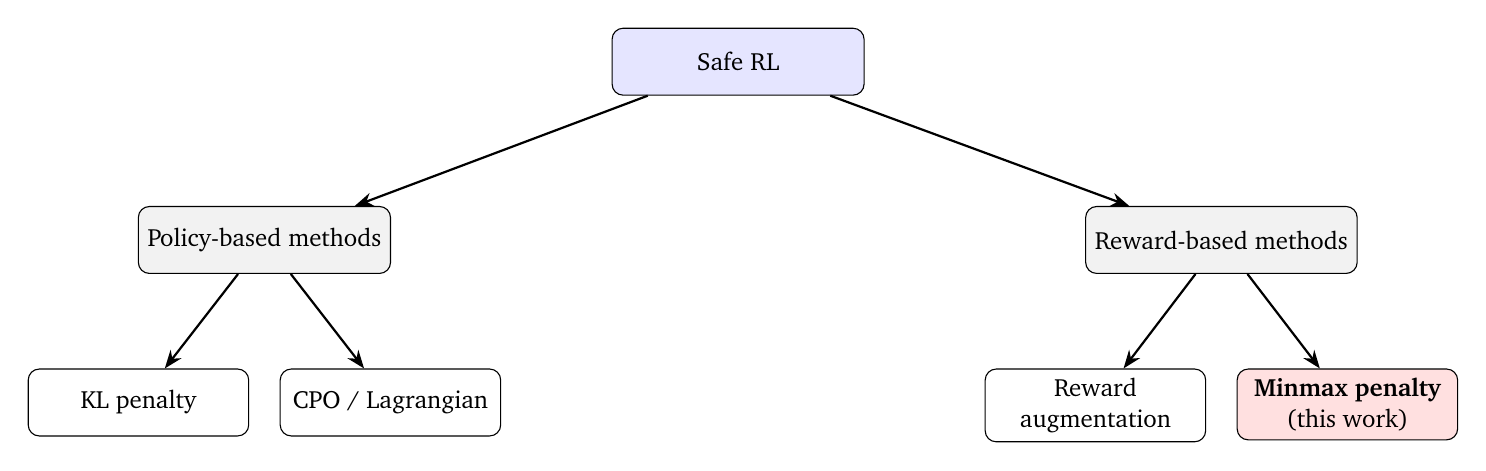
\begin{tikzpicture}[node distance=1.2cm and 2.4cm]
  \node[bblue,  minimum width=3.2cm] (saferl) {Safe RL};
  \node[bgray,  minimum width=3.2cm, below left=1.4cm and 2.8cm of saferl]
    (policy) {Policy-based methods};
  \node[bgray,  minimum width=3.2cm, below right=1.4cm and 2.8cm of saferl]
    (reward) {Reward-based methods};
  \node[block, fill=white, below=1.2cm of policy, xshift=-1.6cm]
    (kl)   {KL penalty};
  \node[block, fill=white, below=1.2cm of policy, xshift= 1.6cm]
    (cpo)  {CPO / Lagrangian};
  \node[block, fill=white, below=1.2cm of reward, xshift=-1.6cm]
    (aug)  {Reward\\augmentation};
  \node[bred,  below=1.2cm of reward, xshift= 1.6cm]
    (mm)   {\textbf{Minmax penalty}\\(this work)};
  \draw[arr] (saferl) -- (policy);
  \draw[arr] (saferl) -- (reward);
  \draw[arr] (policy) -- (kl);
  \draw[arr] (policy) -- (cpo);
  \draw[arr] (reward) -- (aug);
  \draw[arr] (reward) -- (mm);
\end{tikzpicture}}
\caption{Taxonomy of safe RL approaches \citep{garcia2015comprehensive}. The Minmax penalty
  is a reward-based method requiring no learned cost model.}
\label{fig:safe_rl_taxonomy}
\end{figure}

Constrained Policy Optimisation \citep{achiam2017cpo} provides the first policy gradient
method with formal worst-case constraint guarantees:
\begin{equation}
  \pi_{k+1} = \arg\max_\pi J_R(\pi)
  \quad\text{s.t.}\;\; J_{C_i}(\pi) \leq d_i\;\forall i,\quad
  D_{\mathrm{KL}}(\pi\|\pi_k) \leq \delta
  \label{eq:cpo}
\end{equation}
Safe RLHF adapts CPO to the RLHF setting with a learned cost model. Distributional
approaches \citep{yang2022distributional} further strengthen safety by controlling tail-risk
via CVaR. These methods provide the theoretical comparators that motivate asking whether any
constraint model is necessary at all.

\section{Reinforcement Learning with Verifiable Rewards}

A parallel strand of recent work reframes reward design around verifiability: using signals
that can be checked exactly rather than approximated by a learned model
\citep{lambert2024rlvr, youssef2025grpo, su2025crossingreward}. A prominent example is
Group Relative Policy Optimisation (GRPO), introduced by \citet{shao2024deepseekmath} in
DeepSeekMath, which replaces the learned value baseline with group-relative advantages
computed from verifiable mathematical rewards. This eliminates reward model error and
reduces reward hacking. \citet{safetyrlvr2025} study whether such training breaks safety
alignment, finding that KL constraints can preserve safety guardrails. This proposal
investigates the complementary direction: using a deterministically computed, verifiable
value-function signal to actively improve safety rather than merely preserve it.

\section{The ROSARL Algorithm}

ROSARL \citep{nanguetasse2026} proposes that the agent's own value function contains
sufficient information to construct a principled safety penalty without auxiliary models.
At each training step the algorithm maintains $\rmin$ and $\rmax$ as the running minimum
and maximum of all rewards observed so far, and updates value bounds $\vmin$ and $\vmax$
via a three-way minimum and maximum that incorporates both the running reward bounds and
the critic's current value estimate $V(s_t)$: $\vmin \leftarrow \min(\vmin,\rmin,V(s_t))$
and $\vmax \leftarrow \max(\vmax,\rmax,V(s_t))$. This anchoring ensures $\vmin$ tracks the
worst value the agent could plausibly experience and $\vmax$ tracks the best, so that the
penalty gap grows as the agent discovers the full range of achievable values. When the
unsafe-state detector $z_t$ fires, the reward is replaced with
$\runsafe = \vmin - \vmax$, which is always non-positive and lower than the value of any
reachable state under the observed reward and value range. As the agent encounters wider
extremes, $\runsafe$ becomes monotonically more negative, making the penalty more severe
without any manual tuning. \Cref{fig:minmax_dynamics} illustrates this self-calibration
property.

\begin{figure}[ht]
\centering
\resizebox{\linewidth}{!}{%
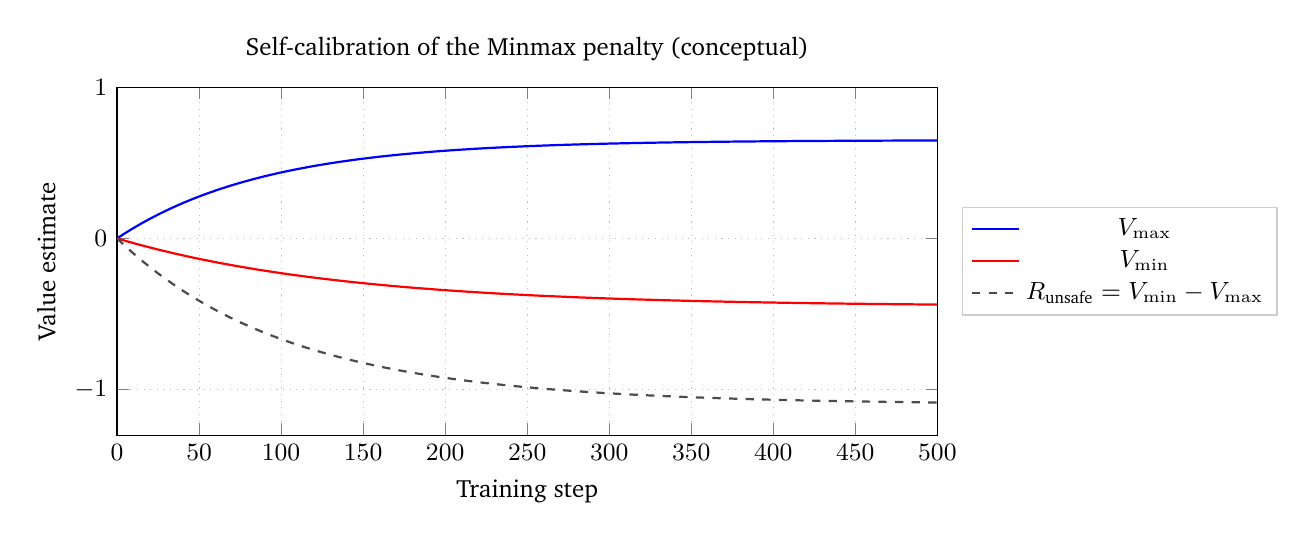
\begin{tikzpicture}
\begin{axis}[
  width=12cm, height=6cm,
  xlabel={Training step},
  ylabel={Value estimate},
  legend style={at={(1.03,0.5)}, anchor=west, font=\small, draw=gray!40},
  grid=major, grid style={dotted,gray!50},
  xmin=0, xmax=500,
  ymin=-1.3, ymax=1.0,
  title style={font=\small},
  title={Self-calibration of the Minmax penalty (conceptual)},
  label style={font=\small},
  tick label style={font=\small}
]
\addplot[blue,  thick, domain=0:500, samples=120]
  { 0.65*(1-exp(-x/90))};
\addlegendentry{$\vmax$}
\addplot[red,   thick, domain=0:500, samples=120]
  {-0.45*(1-exp(-x/140))};
\addlegendentry{$\vmin$}
\addplot[black!70, thick, dashed, domain=0:500, samples=120]
  {-0.45*(1-exp(-x/140)) - 0.65*(1-exp(-x/90))};
\addlegendentry{$\runsafe = \vmin - \vmax$}
\end{axis}
\end{tikzpicture}}
\caption{Conceptual illustration of the self-calibration property. As training progresses
  $\runsafe$ becomes monotonically more negative, providing increasingly strong corrective
  signal without any manual tuning.}
\label{fig:minmax_dynamics}
\end{figure}

ROSARL was validated on Safety-Gymnasium benchmarks (PointGoal, PointPush,
HumanoidVelocity, PILLAR) and matches or outperforms Lagrangian, CPO, and Sauté-RL baselines
under environmental stochasticity. This proposal is the first application to LLM fine-tuning.

\section{Datasets}

This section describes the datasets used for training and evaluation in this research.

\textbf{BeaverTails} \citep{ji2023beavertails} is a large-scale human preference dataset
covering 14 harm categories: animal abuse, child abuse, controversial topics, discrimination,
drug abuse, financial crime, hate speech, human rights violations, non-violent unethical
behaviour, privacy violations, sexually explicit content, terrorism, violence, and weapons.
Uniquely, it provides separate annotations for helpfulness and harmlessness for the same
prompt. The training split (27,186 prompts) is used for fine-tuning; the held-out
BeaverTails-Evaluation split (700 prompts) serves as the primary evaluation benchmark,
shared with Safe RLHF and HC-RLHF to enable direct SOTA comparison.

\textbf{PKU-SafeRLHF} \citep{ji2024pkusaferlhf} extends BeaverTails with multi-level safety
labels across 19 harm categories and three severity levels, providing paired safe and unsafe
responses for the same prompts. This structure is directly relevant to the Phase 2 extension:
the paired responses provide explicit positive and negative training examples for the
activation probe.

\textbf{HarmBench} \citep{mazeika2024} provides over 500 unique adversarial harmful
behaviours designed to probe LLM safety under worst-case conditions. Unlike BeaverTails,
which covers naturalistic prompts, HarmBench is specifically designed for red-teaming: it
includes standard, contextual, and multi-turn behaviours, as well as attacks that span
multiple harm categories simultaneously. In this research, HarmBench serves as an
out-of-distribution robustness evaluation, testing whether the Minmax penalty generalises
beyond the harm categories and prompt styles seen during BeaverTails training. Full
HarmBench evaluation is planned as a later milestone pending larger model access.

\section{Activation-Based Safety Detection}

This section reviews the activation-based safety detection literature that motivates Phase 2
of this research.

\citet{rateike2023} demonstrate that LLMs encode unsafe information in internal activation
vectors during generation, before the output token is produced. Using DeepScan (subset
scanning), they identify specific neuron subsets in the final layers of OPT-6.7B that are
anomalously active when the model is about to hallucinate. Crucially, hallucination detection
was found to be the most tractable starting subset for detection, a finding from recent
follow-up work currently under review that directly informs the Phase 2 design: the
activation probe will target factually incorrect outputs first before extending to broader
harm categories. \citet{cintas2025} extend this to persona representations in decoder-only
LLMs, finding that safety-relevant representations are localised in the final third of
layers, with the open question of whether these activations can steer generation.

SafeSwitch \citep{han2025safeswitch} provides the most direct empirical precedent for
Phase 2: internal activation signals can directly steer unsafe behaviour in deployed LLMs,
achieving large reductions in harmful outputs while preserving utility. SafetyNet
\citep{chaudhary2025safetynet} provides complementary evidence by monitoring deceptive
behavioural signals in activations in real time. \citet{nguyen2025distributional} further
show that distributional surgery on activations can both detect and mitigate undesirable
content layerwise.


% =============================================================================
\chapter{Research Methodology}
\label{ch:methodology}
% =============================================================================

This chapter describes the full experimental design in two phases.
Section~\ref{sec:problem-statement} states the problem this research addresses.
Section~\ref{sec:research-questions} specifies the research questions and the hypotheses
that structure the experimental programme. Section~\ref{sec:methodology} details the
methodology, including data collection (Section~\ref{sec:data-collection}), the two-phase
pipeline architecture (Section~\ref{sec:pipeline}), the ablation design
(Section~\ref{sec:ablations}), and the limitations and constraints that bound the scope of
claims (Section~\ref{sec:limitations}).

\section{Problem Statement}
\label{sec:problem-statement}

LLMs fine-tuned with PPO can produce harmful outputs at deployment at rates that undermine
their trustworthiness in safety-critical applications \citep{dai2024saferlhf,
chittepu2025}. Current mitigation strategies each introduce a structural cost: KL
divergence penalties require manual tuning of the KL coefficient and trade safety against
capability without a principled basis for setting the trade-off; learned cost models
require a second trained model, additional harmlessness annotations, and a Lagrangian
multiplier whose update dynamics introduce further hyperparameter burden. These mechanisms
add components external to the core PPO loop, increasing engineering and annotation cost
without providing a principled safety guarantee. This research addresses the question of
whether the value function already present in the PPO training loop can itself supply a
self-calibrating safety signal that replaces both mechanisms. The methodology in
Section~\ref{sec:methodology} operationalises this question through Algorithm~1, ablation
studies that isolate the Minmax mechanism, and a two-phase pipeline that varies only the
unsafe-state detector.

\section{Research Questions}
\label{sec:research-questions}

This research investigates whether the ROSARL Minmax penalty can serve as the primary
safety mechanism in PPO-based LLM fine-tuning, replacing KL divergence penalties and
learned cost models, across multiple base models and fine-tuning strategies. The
experimental programme is structured around three hypotheses; each hypothesis maps
directly to one dimension of the ablation design described in
Section~\ref{sec:ablations}, so that the three together cover the safety mechanism, the
detector, and the architectural extension to activation-level detection.

\begin{itemize}
  \item \textbf{H1 (mechanism).} A policy trained with the Minmax penalty produces fewer
    harmful outputs than a policy trained with KL divergence alone, measured by harm rate
    on BeaverTails-Evaluation. This effect is expected to persist across base models
    (GPT-2 small and a small Qwen model) and fine-tuning strategies (full fine-tuning and
    LoRA), isolating the mechanism as the source of the benefit rather than any
    model-specific property.
  \item \textbf{H2 (detector quality bounds coverage).} The Minmax penalty's harm
    reduction is bounded by the recall of the unsafe-state detector. Categories where the
    detector signal is weak or absent, such as self-harm under Detoxify, are not expected
    to improve and may regress, because Algorithm~1 only acts when $z_t = 1$. This frames
    detector quality as the primary variable modulating coverage, not the penalty
    mechanism itself.
  \item \textbf{H3 (consequence of H2).} If H2 holds, then replacing Detoxify with an
    activation-level probe should extend coverage to categories where Detoxify's recall is
    near zero (most notably self-harm), without altering the underlying Minmax mechanism.
    H3 tests this prediction directly: the penalty is held fixed, only the source of $z_t$
    is varied, so that any change in coverage is attributable to the detector rather than
    to a different safety algorithm.
\end{itemize}

\section{Methodology}
\label{sec:methodology}

This section details the experimental methodology. PPO is used for all fine-tuning runs,
comparing a KL-penalty baseline against the Minmax penalty. The unsafe-state detector is
Detoxify in Phase 1 and an activation-based probe in Phase 2. Evaluation is performed on
two benchmarks: BeaverTails-Evaluation \citep{ji2023beavertails} as the in-distribution
harm-rate measure, and HarmBench \citep{mazeika2024} as an out-of-distribution adversarial
robustness measure. Ablations isolate the effect of the Minmax mechanism from confounds
such as base model, fine-tuning strategy, and detector threshold. The methodology is
structured around four components: data collection (Section~\ref{sec:data-collection}),
the two-phase pipeline architecture (Section~\ref{sec:pipeline}), ablation studies
(Section~\ref{sec:ablations}), and limitations and constraints
(Section~\ref{sec:limitations}).

\subsection{Data Collection}
\label{sec:data-collection}

To compare the Minmax penalty with existing methods, PPO fine-tuning with the Minmax
penalty is implemented on GPT-2 small and a small Qwen model. The training split of
BeaverTails is used for fine-tuning, with evaluation on the held-out BeaverTails-Evaluation
split and on HarmBench.

\paragraph{Implementation framework.}
The primary implementation framework is the TRL library's \texttt{PPOTrainer}
\citep{vonwerra2022trl}, into which the Minmax penalty is integrated as a reward
wrapper following the structure of Algorithm~\ref{alg:minmax}. The PKU-SafeRLHF
codebase \citep{ji2024pkusaferlhf} is used as the reference implementation for
understanding the Safe RLHF baseline design, not as the running framework: it
requires DeepSpeed, which does not build on the available Windows hardware. A
later milestone will port the Minmax wrapper into the PKU-SafeRLHF codebase on a
Linux cluster to enable direct head-to-head comparison with the published Safe RLHF
and HC-RLHF baselines under matched infrastructure.

\paragraph{Algorithm~1 Implementation.}
The Minmax penalty is implemented as a reward wrapper around the TRL
\texttt{PPOTrainer} \citep{vonwerra2022trl}. The full procedure is given in
Algorithm~\ref{alg:minmax}.

\begin{algorithm}[H]
\caption{PPO + Minmax Penalty (LLM adaptation of ROSARL \citep{nanguetasse2026})}
\label{alg:minmax}
\begin{algorithmic}[1]
\Require LLM $\pi_\theta$, critic $V_\psi$, unsafe detector $\mathcal{D}$, threshold $\tau$, KL anchor $\beta$
\State Initialise $\rmin \leftarrow 0,\; \rmax \leftarrow 0,\; \vmin \leftarrow 0,\; \vmax \leftarrow 0$ \Comment{as in original ROSARL}
\For{each training step $t$}
  \State Sample prompt $x \sim \mathcal{X}_{\text{train}}$
  \State Generate response $y \sim \pi_\theta(\cdot \mid x)$
  \State $\delta_t \leftarrow \mathcal{D}(y)$ \Comment{detector score}
  \State $r^{\text{raw}}_t \leftarrow -\delta_t$ \Comment{raw reward (LLM adaptation: negated Detoxify score)}
  \State $V_t \leftarrow V_\psi(x, y)$ \Comment{critic value estimate}
  \State $\rmin \leftarrow \min(\rmin,\, r^{\text{raw}}_t)$;\quad $\rmax \leftarrow \max(\rmax,\, r^{\text{raw}}_t)$ \Comment{ROSARL reward bounds}
  \State $\vmin \leftarrow \min(\vmin,\, \rmin,\, V_t)$;\quad $\vmax \leftarrow \max(\vmax,\, \rmax,\, V_t)$ \Comment{ROSARL three-way value bounds}
  \If{$\delta_t > \tau$} \Comment{unsafe state detected}
    \State $r_t \leftarrow \max(\vmin - \vmax,\; -1.0)$ \Comment{Minmax penalty; $-1.0$ floor is a stabilisation modification, not in original ROSARL}
  \Else
    \State $r_t \leftarrow r^{\text{raw}}_t$ \Comment{LLM adaptation: detector reward (original uses environment reward)}
  \EndIf
  \State Update $\pi_\theta$, $V_\psi$ via PPO with $r_t$ and KL penalty $\beta$
\EndFor
\end{algorithmic}
\end{algorithm}

Key design choices, with explicit attribution to either ROSARL or this work:
\begin{itemize}
  \item \textbf{Reward-bound tracking ($\rmin$, $\rmax$) and the $\runsafe = \vmin - \vmax$ formula} are taken unchanged from ROSARL \citep{nanguetasse2026}.
  \item \textbf{Three-way value-bound update.} Following Algorithm~1 of
    \citet{nanguetasse2026}, $\vmin$ and $\vmax$ are updated using a three-way
    minimum and maximum respectively: $\vmin$ incorporates both the running minimum
    reward $\rmin$ and the critic's current value estimate $V(s_t)$, ensuring the
    penalty gap grows as the agent discovers the full range of achievable values.
    $\vmax$ is correspondingly anchored to the highest reward and value seen,
    providing an optimistic upper bound that makes $\runsafe$ conservative by
    construction.
  \item \textbf{The $-1.0$ floor on the unsafe reward} is not part of the original
    Algorithm~1; it was introduced as an engineering modification to guard against
    catastrophic PPO ratio violations during early training, when value estimates are
    not yet well-calibrated and $\vmin - \vmax$ can briefly take very large negative
    values.
  \item \textbf{The safe-branch reward $r_t \leftarrow -\delta_t$} is this work's
    LLM-setting adaptation: in the absence of a dense environment reward signal, the
    negated Detoxify toxicity score provides a continuous signal that the policy can
    optimise, encouraging progressively less toxic outputs even when no unsafe flag
    is triggered. This differs from the original Algorithm~1, in which the
    environment reward is passed through unchanged for safe transitions.
  \item \textbf{The small KL anchor ($\beta = 0.01$)} is retained solely to prevent
    mode collapse and is distinct from the $\beta = 0.2$ used in the KL baseline
    condition.
  \item \textbf{Reducing PPO epochs from 4 to 1} prevents the probability ratio from
    exploding when the reward sign flips abruptly between the safe and unsafe branches.
\end{itemize}

\paragraph{Base models and fine-tuning strategies.}
GPT-2 small (117M parameters) serves as the primary base model, feasible on the
available hardware. A Qwen model in the 1 to 3B parameter range is planned for the
model-scale ablation (Ablation~2), to be run on a compute cluster. LoRA
\citep{hu2022lora} is used as the fine-tuning strategy for larger models, as it reduces
memory requirements while still permitting comparison across fine-tuning methods in
Ablation~3. In Phase 1, Detoxify \citep{hanu2020detoxify} provides the binary signal
$z_t$ indicating whether the model output is classified as harmful. In Phase 2, Detoxify
is replaced with an activation-based probe targeting hallucination detection as the
initial subset, following the methodology of \citet{rateike2023}.

\paragraph{Evaluation benchmarks.}
The primary evaluation benchmark is the held-out BeaverTails-Evaluation set (700 prompts
across 14 harm categories). Both trained models generate 32 tokens per prompt; outputs are
classified as harmful or benign, and harm rate is reported in aggregate and by category,
enabling direct comparison with published Safe RLHF \citep{dai2024saferlhf} and HC-RLHF
\citep{chittepu2025} results, which use the same split. The secondary benchmark is
HarmBench \citep{mazeika2024}, which provides over 500 adversarial behaviours specifically
designed for red-teaming, spanning standard, contextual, and multi-turn attacks that cross
harm categories. Evaluation on HarmBench tests whether the Minmax penalty generalises
beyond the naturalistic BeaverTails prompts seen during training. Following
\citet{mazeika2024}, attack success rate (ASR) is the primary metric, reported overall and
broken down by attack family. HarmBench evaluation is planned as a later phase, after
Phase 1 results are stable.

\subsection{Pipeline Implementation: Two-Phase Architecture}
\label{sec:pipeline}

The research is structured in two phases, each defined by the unsafe-state detector that
feeds the binary signal $z_t$ into Algorithm~1. In both phases the PPO training loop and
the Minmax penalty itself are identical; only the source of $z_t$ changes. The two phases
are illustrated in \Cref{fig:phase1} and \Cref{fig:phase2}.

\textbf{Phase 1: Detoxify as the unsafe-state detector.} At each training step a prompt
$x$ is drawn from BeaverTails and the policy $\pi_\theta$ generates a response $y$.
Detoxify \citep{hanu2020detoxify} scores $y$ and returns a toxicity probability
$\delta_t \in [0,1]$; the binary signal is $z_t$. The Minmax wrapper then sets the
per-trajectory reward to $\runsafe = \vmin - \vmax$ whenever $z_t = 1$, and to the
standard reward $-\delta_t$ otherwise, before passing it to the PPO update. This phase is
the focus of the empirical evaluation in this proposal: it requires no additional training
of a safety model, and produces a fast feedback loop that makes the core Minmax claim
falsifiable on BeaverTails-Evaluation and HarmBench. \Cref{fig:phase1} shows the Phase 1
architecture.

\begin{figure}[H]
\centering
\resizebox{\linewidth}{!}{%
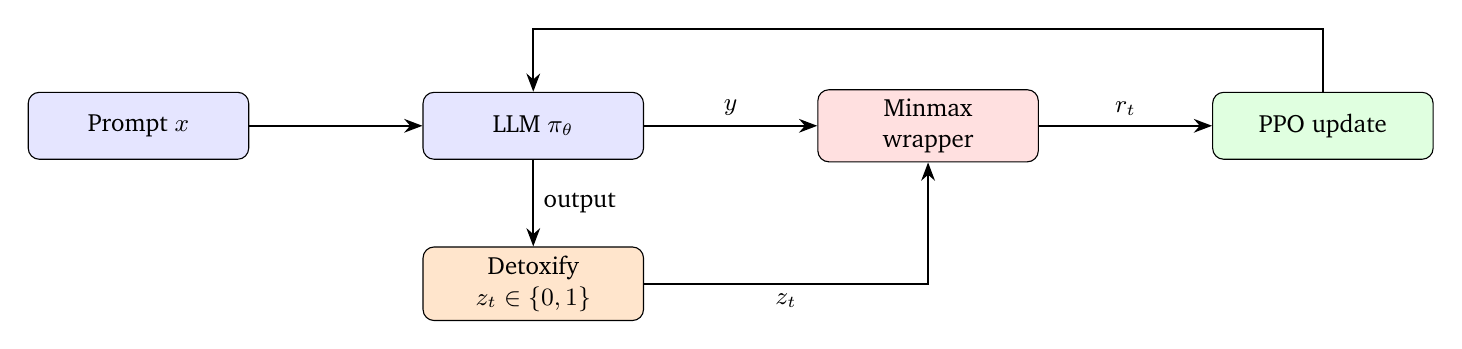
\begin{tikzpicture}[node distance=0.9cm and 2.2cm]
  \node[bblue]  (prompt)  {Prompt $x$};
  \node[bblue,  right=2.2cm of prompt]  (llm)    {LLM $\pi_\theta$};
  \node[borange,below=1.1cm of llm]     (dtox)   {Detoxify\\$z_t \in \{0,1\}$};
  \node[bred,   right=2.2cm of llm]     (mm)     {Minmax\\wrapper};
  \node[bgreen, right=2.2cm of mm]      (ppo)    {PPO update};
  \draw[arr] (prompt) -- (llm);
  \draw[arr] (llm)    -- node[above]{\small$y$} (mm);
  \draw[arr] (llm)    -- node[right]{\small output} (dtox);
  \draw[arr] (dtox)   -| node[below, near start]{\small$z_t$} (mm);
  \draw[arr] (mm)     -- node[above]{\small$r_t$} (ppo);
  \draw[arr] (ppo.north) -- ++(0,0.8) -| node[above, near end]{} (llm.north);
\end{tikzpicture}}
\caption{Phase 1 architecture. Detoxify classifies the model output, providing the binary
  unsafe flag $z_t$ to the Minmax wrapper. When $z_t=1$, the wrapper replaces the reward
  with $\runsafe = \vmin - \vmax$ before passing it to the PPO update.}
\label{fig:phase1}
\end{figure}

\textbf{Phase 2: Activation probe as the unsafe-state detector.} Phase 2 keeps the rest of
the pipeline fixed and replaces Detoxify with a lightweight activation probe trained on
internal model states, following \citet{rateike2023, han2025safeswitch}. The motivation is
that surface-level classifiers cannot detect categories such as self-harm, where the
output is fluent and non-toxic but the underlying intent is unsafe. Phase 2 is a planned
extension scoped as a single milestone; a detailed design is deferred until Phase 1
results are stable. \Cref{fig:phase2} shows the Phase 2 architecture.

\begin{figure}[H]
\centering
\resizebox{\linewidth}{!}{%
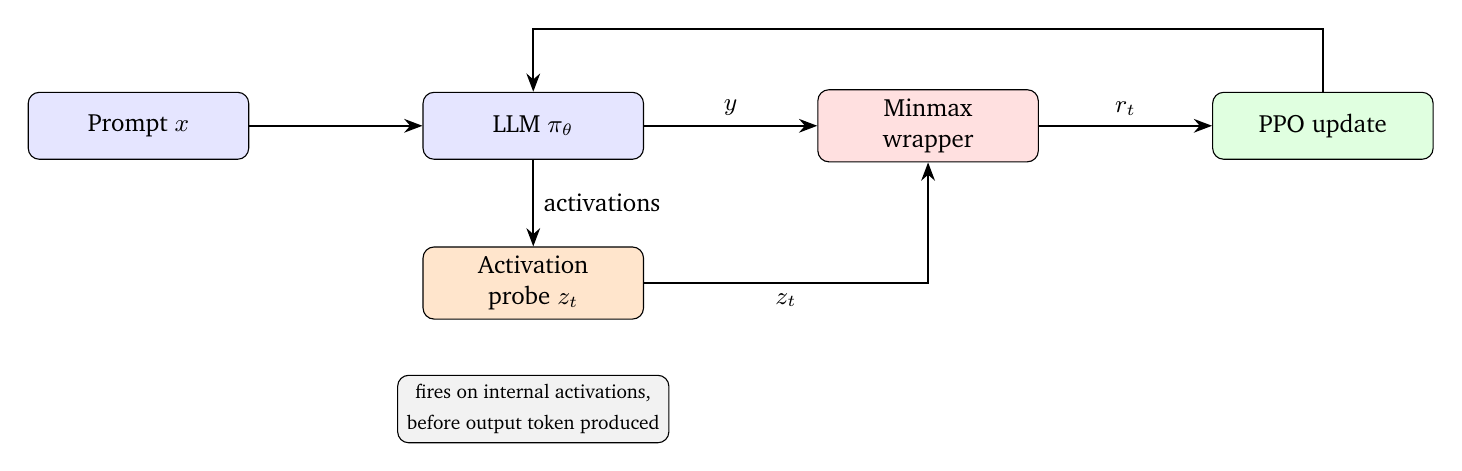
\begin{tikzpicture}[node distance=0.9cm and 2.2cm]
  \node[bblue]  (prompt)  {Prompt $x$};
  \node[bblue,  right=2.2cm of prompt]  (llm)    {LLM $\pi_\theta$};
  \node[borange,below=1.1cm of llm]     (probe)  {Activation\\probe $z_t$};
  \node[bred,   right=2.2cm of llm]     (mm)     {Minmax\\wrapper};
  \node[bgreen, right=2.2cm of mm]      (ppo)    {PPO update};
  \node[bgray,  below=0.7cm of probe]   (note)
    {\scriptsize fires on internal activations,\\
     \scriptsize before output token produced};
  \draw[arr] (prompt) -- (llm);
  \draw[arr] (llm)    -- node[above]{\small$y$} (mm);
  \draw[arr] (llm)    -- node[right]{\small activations} (probe);
  \draw[arr] (probe)  -| node[below, near start]{\small$z_t$} (mm);
  \draw[arr] (mm)     -- node[above]{\small$r_t$} (ppo);
  \draw[arr] (ppo.north) -- ++(0,0.8) -| node[above, near end]{} (llm.north);
\end{tikzpicture}}
\caption{Phase 2 architecture. The activation probe replaces Detoxify, detecting unsafe
  states from internal activations before the output token is produced. This extends
  Algorithm~1's coverage to harm categories that surface-level classifiers miss.}
\label{fig:phase2}
\end{figure}

\textbf{Evaluation across both phases.} Trained policies are evaluated on two
complementary benchmarks. The primary, in-distribution benchmark is
BeaverTails-Evaluation: 700 held-out prompts across 14 harm categories. Both trained
models generate 32 tokens per prompt; outputs are classified as harmful or benign, and
harm rate is reported in aggregate and per category. Using the same split as Safe RLHF
\citep{dai2024saferlhf} and HC-RLHF \citep{chittepu2025} enables direct comparison with
published results.

The secondary, out-of-distribution benchmark is HarmBench \citep{mazeika2024}, which
provides over 500 adversarial behaviours designed for red-teaming, spanning standard,
contextual, and multi-turn attacks that cross harm categories. HarmBench tests whether the
Minmax penalty generalises beyond the naturalistic BeaverTails prompts seen during
training, and is the stronger test of $H_1$: a method that only reduces harm on
in-distribution prompts could simply be reproducing the training distribution rather than
learning a robust safety policy. Following \citet{mazeika2024}, attack success rate (ASR)
is the primary metric, reported overall and broken down by attack family. Full HarmBench
evaluation is run after Phase 1 results are stable, and again after Phase 2.

At each training step the following are logged: mean reward, $\vmin$, $\vmax$,
$\runsafe$, policy KL divergence, and PPO ratio statistics, enabling inspection of the
self-calibration dynamics predicted by \citet{nanguetasse2026}. Ablations on safety
mechanism, base model, fine-tuning strategy, and detector threshold isolate the
contribution of the Minmax mechanism from confounds (see Section~\ref{sec:ablations}).

\subsection{Ablation Studies}
\label{sec:ablations}

The ablation design is structured to isolate the Minmax mechanism as the causal factor for
any observed safety improvement, varying one dimension at a time while holding all others
fixed. This is essential to rule out confounds from the choice of base model, fine-tuning
strategy, or detector sensitivity.

\textbf{Ablation 1: Safety mechanism.} The core comparison, holding everything fixed and
varying only the safety mechanism: PPO with KL penalty (baseline), PPO with Minmax
(proposed), and PPO with no safety mechanism (lower bound).

\textbf{Ablation 2: Base model.} Holds the Minmax mechanism fixed and varies the base
model between GPT-2 small (hardware-feasible) and a Qwen model at 1 to 3B parameters
(cluster). This directly addresses the concern that the observed improvement might be
specific to GPT-2 rather than attributable to the Minmax mechanism.

\textbf{Ablation 3: Fine-tuning method.} Holds the Minmax mechanism and base model fixed
and varies the fine-tuning strategy between full fine-tuning and LoRA. This addresses the
concern that the result might be confounded by the training approach rather than the safety
mechanism.

\textbf{Ablation 4: Detector threshold.} Holds all other parameters fixed and varies the
unsafe threshold $\tau \in \{0.1, 0.3, 0.5, 0.7\}$ to characterise how detector sensitivity
affects harm rate and policy stability.

Extended training runs of 1000 to 2000 steps will confirm whether results from the 500-step
pilot are stable over longer training.

\subsection{Limitations and Constraints}
\label{sec:limitations}

This research is bounded by several constraints that shape the scope of claims that can be
made from its results.

\textbf{Detector quality bounds coverage.} By construction, Algorithm~1 only acts when the
unsafe-state detector fires. In Phase 1, this couples the achievable harm reduction to
Detoxify's recall: harm categories whose surface form does not register as toxic (most
notably self-harm) cannot be improved by the Minmax penalty regardless of how well-tuned
the RL loop is. This is the explicit motivation for Phase 2, but it remains a constraint on
Phase 1 results.

\textbf{Benchmark coverage.} BeaverTails-Evaluation and HarmBench together cover
naturalistic and adversarial harm but do not exhaust the space of safety-relevant
behaviours; truthfulness and long-horizon manipulation are not directly measured. HarmBench
evaluation depends on access to its judge classifier and is therefore scheduled as a later
milestone.

\textbf{Phase 2 scope.} The activation-probe extension is scoped as a single milestone with
hallucination as the initial target subset, following \citet{rateike2023}. A full study of
probe architectures and layer selection is identified as future work.

\textbf{Statistical scope.} The proof-of-concept reported in Chapter~\ref{ch:prelim} is a
single 500-step run per condition. The full experimental programme will use multiple seeds
per condition so that reported harm-rate differences can be tested for significance rather
than reported as point estimates.

% =============================================================================
\chapter{Preliminary Results}
\label{ch:prelim}
% =============================================================================

The results in this chapter are from a 500-step proof-of-concept pilot on GPT-2 small. They
are not the primary experimental results of this thesis. Their purpose is to demonstrate
that Algorithm~1 is compatible with the TRL PPOTrainer implementation, that it produces a
measurable safety signal in the LLM setting, and to provide early evidence of feasibility
that motivates the full experimental programme.

\section{Overall Harm Rate}

\Cref{tab:results} and \Cref{fig:harm_rate_bar} show the overall harm rate on
BeaverTails-Evaluation. The Minmax penalty produced a 58.7\% relative reduction in harm rate
over the KL-only baseline, providing initial support for H1.

\begin{table}[ht]
  \centering
  \caption{Proof-of-concept pilot: harm rate on BeaverTails-Evaluation (700 prompts).}
  \label{tab:results}
  \begin{tabular}{lccc}
    \toprule
    \textbf{Condition} & \textbf{Harm Rate} & \textbf{Harmful / Total} & \textbf{Reduction} \\
    \midrule
    GPT-2 + PPO + KL (baseline)        & 17.29\% & 121/700 & \\
    GPT-2 + PPO + Minmax (Algorithm~1) & 7.14\%  & 50/700  & 58.7\% relative \\
    \bottomrule
  \end{tabular}
\end{table}

\begin{figure}[ht]
\centering
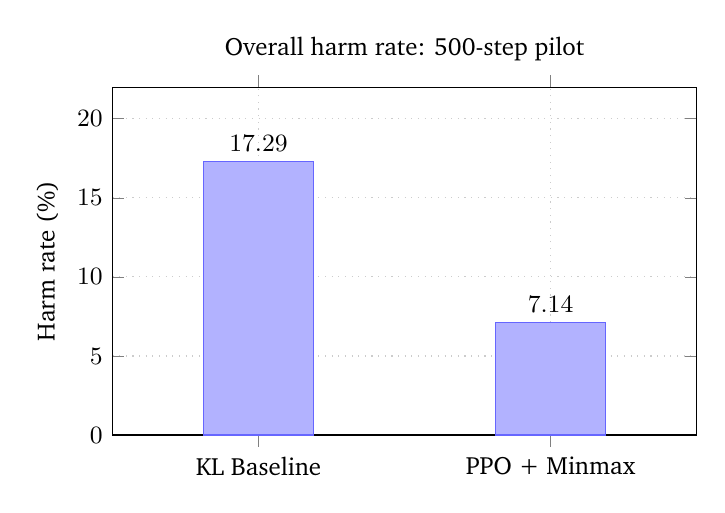
\begin{tikzpicture}
\begin{axis}[
  ybar,
  width=9cm, height=6cm,
  bar width=1.4cm,
  ylabel={Harm rate (\%)},
  symbolic x coords={KL Baseline, PPO + Minmax},
  xtick=data,
  ymin=0, ymax=22,
  nodes near coords,
  nodes near coords align={vertical},
  every node near coord/.append style={font=\small},
  grid=major, grid style={dotted,gray!40},
  title={Overall harm rate: 500-step pilot},
  title style={font=\small},
  label style={font=\small},
  tick label style={font=\small},
  enlarge x limits=0.5
]
\addplot[fill=blue!30, draw=blue!60]
  coordinates {(KL Baseline,17.29) (PPO + Minmax,7.14)};
\end{axis}
\end{tikzpicture}
\caption{Overall harm rate on BeaverTails-Evaluation (700 prompts). The Minmax penalty
  produces a 58.7\% relative reduction compared to the KL-penalty baseline.}
\label{fig:harm_rate_bar}
\end{figure}

\section{Per-Category Analysis}

\Cref{tab:percategory} breaks down results by harm category. Categories where Detoxify
reliably detects toxic language, such as discrimination and hate speech, show large
improvements. The self-harm regression (+10pp) is the most informative finding: self-harm
prompts use clinical, neutral language that Detoxify scores as low toxicity (approximately
0.01 to 0.05), so $z_t$ never fires and Algorithm~1 has no signal to act on. This confirms
H2 and directly motivates the Phase 2 activation probe extension.

\begin{table}[ht]
  \centering
  \caption{Per-category harm rate: 500-step pilot.}
  \label{tab:percategory}
  \begin{tabular}{lcccc}
    \toprule
    \textbf{Harm Category} & \textbf{Baseline} & \textbf{Minmax}
      & \textbf{$\Delta$ (pp)} & \textbf{Result} \\
    \midrule
    Discrimination / stereotype          & 46\% & 8\%  & $-38$ & \checkmark\checkmark \\
    Hate speech / offensive language     & 46\% & 12\% & $-34$ & \checkmark\checkmark \\
    Animal abuse                         & 36\% & 16\% & $-20$ & \checkmark \\
    Child abuse                          & 22\% & 4\%  & $-18$ & \checkmark \\
    Sexually explicit                    & 46\% & 30\% & $-16$ & $\sim$ \\
    Privacy violation                    & 14\% & 2\%  & $-12$ & \checkmark \\
    Controversial topics / politics      & 10\% & 4\%  & $-6$  & \checkmark \\
    Self-harm                            & 8\%  & 18\% & $+10$ & $\times$ \\
    Drug abuse / weapons                 & 0\%  & 0\%  & 0     & $=$ \\
    \bottomrule
  \end{tabular}
\end{table}

\section{Training Dynamics}

The self-calibration behaviour predicted by \citet{nanguetasse2026} was broadly observed in
the training logs: $\vmax$ grew positive within the first 10 steps; $\vmin$ went negative
within 10 steps; $\runsafe$ grew more negative across 500 steps. No catastrophic PPO ratio
violations were observed after reducing PPO epochs from 4 to 1.

One known characteristic of the pilot run is that $\vmin$ remained closer to 0 than
expected, because GPT-2 mostly generates clean text on BeaverTails prompts and the
critic's value estimates did not reach strongly negative territory during the 500 training
steps. This is consistent with the self-calibration property of Algorithm~1 in a low-harm
regime and is not a fundamental issue with the mechanism: longer extended runs in the full
experimental programme are expected to widen $\vmin$ as the policy explores a broader
response distribution.

% =============================================================================
\chapter{Research Plan}
\label{ch:plan}
% =============================================================================

This chapter outlines the planned experimental phases, target results, success criteria, and
proposed future extension.

\section{Timeline}

The planned phases are summarised in \Cref{tab:timeline}, with indicative month ranges
relative to the project start in May 2026 and the standard two-year MSc duration. The
500-step proof-of-concept pilot reported in Chapter~\ref{ch:prelim} is complete; all other
phases are planned. Cluster-dependent phases (Qwen model scale, HarmBench evaluation) are
scheduled after cluster access is confirmed.

\begin{table}[ht]
  \centering
  \caption{Indicative timeline. Month ranges are relative to project start (May 2026).}
  \label{tab:timeline}
  \begin{tabular}{clcc}
    \toprule
    \textbf{Phase} & \textbf{Activities} & \textbf{Months} & \textbf{Status} \\
    \midrule
    1 & Proposal submission and ethics clearance & 1--2 & In progress \\
    2 & Full Phase 1 GPT-2 runs (extended steps, ablations) & 2--4 & Planned \\
    3 & LoRA fine-tuning experiments; threshold ablation & 4--5 & Planned \\
    4 & Qwen model scale experiments (cluster) & 5--7 & Planned \\
    5 & Phase 2 activation probe preliminary experiment & 7--9 & Planned \\
    6 & HarmBench out-of-distribution evaluation & 9--10 & Planned \\
    7 & Thesis writing and submission & 10--24 & Planned \\
    \bottomrule
  \end{tabular}
\end{table}

\section{Target Results}

\begin{table}[ht]
  \centering
  \caption{Target results table for thesis. [TBD] entries are planned experiments.}
  \label{tab:target}
  \scalebox{0.92}{
  \begin{tabular}{lccc}
    \toprule
    \textbf{Condition}
      & \textbf{Harm Rate $\downarrow$}
      & \textbf{Mean Reward $\uparrow$}
      & \textbf{Notes} \\
    \midrule
    GPT-2 zero-shot              & [TBD]    & [TBD]  & Untrained baseline \\
    PPO + KL (pilot)             & 17.29\%  & 0.9980 & Done \\
    PPO + Minmax (pilot)         & 7.14\%   & 0.7995 & Done \\
    PPO + Minmax (extended)      & [TBD]    & [TBD]  & Extended training \\
    PPO + Minmax (LoRA)          & [TBD]    & [TBD]  & Fine-tuning ablation \\
    Qwen + Minmax                & [TBD]    & [TBD]  & Model scale ablation \\
    Safe RLHF 7B (from paper)    & 1--3\%   & N/A    & SOTA \citep{dai2024saferlhf} \\
    HC-RLHF (from paper)         & [reported] & N/A  & Newest SOTA \citep{chittepu2025} \\
    \bottomrule
  \end{tabular}}
\end{table}

\section{Success Criteria}

\textbf{Minimum bar.} Reproduce the pilot harm rate reduction on a clean run. Extended
training shows stable or improving safety performance. Ablation studies document sensitivity
to threshold, KL anchor, fine-tuning method, and base model. Per-category analysis clearly
attributes the self-harm regression to detector quality.

\textbf{Target.} All minimum criteria, plus: final BeaverTails-Evaluation results
competitive with published baselines at comparable model scale; Phase 2 activation probe
experiment showing that the self-harm signal is detectable in GPT-2 activations (or
providing a clear null result); and HarmBench \citep{mazeika2024} evaluation for
out-of-distribution robustness.

\section{Proposed Future Extension}

The self-harm regression motivates Phase 2: replacing Detoxify with an activation probe
trained to detect unsafe internal states before the output token is produced. Based on
\citet{rateike2023}'s finding that hallucination detection is the most tractable initial
subset, the probe will first target factually incorrect and internally inconsistent outputs.
The PKU-SafeRLHF dataset \citep{ji2024pkusaferlhf}, with its paired safe and unsafe
responses across 19 harm categories, provides explicit positive and negative training
examples for the probe. Once validated on hallucination detection, the probe will be extended
to self-harm and other categories that Detoxify misses, directly answering the open question
posed by \citet{cintas2025}.

% =============================================================================
\chapter{Conclusion}
\label{ch:conclusion}
% =============================================================================

This proposal presents a research programme investigating whether the ROSARL Minmax penalty
can serve as the primary safety mechanism in PPO-based LLM fine-tuning, replacing both KL
divergence penalties and learned cost models. The central motivation is that the RL loop
already contains the information needed for safe behaviour, in the form of the actor-critic
algorithm's own value function, and that adding external mechanisms may not be necessary.

Early proof-of-concept evidence is encouraging, and the per-category findings provide a
clear research direction: the penalty mechanism appears sound, and detector quality is the
primary variable modulating coverage. The two-phase architecture, moving from surface-level
toxicity detection to activation-based safety signals, is designed to address this directly.
The planned ablation programme, varying base model, fine-tuning strategy, and detector
threshold, will establish whether observed improvements are attributable to the Minmax
mechanism rather than to any specific experimental configuration.

A successful thesis outcome, completing both phases, confirming mechanism-specificity
through the ablations, and demonstrating that Phase 2 extends coverage to categories such
as self-harm, would contribute to the safe RLHF literature a concrete demonstration that
value-function-derived signals can replace both KL penalties and learned cost models, and
that the binding constraint on safety coverage is detector quality rather than algorithm
design. This places the Minmax penalty within the emerging RL with verifiable rewards
paradigm \citep{lambert2024rlvr, shao2024deepseekmath, safetyrlvr2025}: the signal is
computed deterministically from the agent's own training trajectory rather than
approximated by a learned model. For practitioners, the approach is attractive because it
requires no additional annotation, no separate trained model, and no new safety-specific
hyperparameters, making it accessible to teams working within tight compute budgets and
providing a path toward safer PPO-based fine-tuning that does not depend on access to
large annotation pipelines.

\addcontentsline{toc}{chapter}{References}
\bibliography{references}

\end{document}